\documentclass{article}
\usepackage{geometry}
\usepackage{amsmath}
\usepackage{pgfplots} 
\usepackage{graphicx}
\usepackage[utf8]{inputenc}
\usepackage[brazil]{babel}
\usepackage[dvipsnames]{xcolor}
\newcommand{\highlight}[1]{\colorbox{yellow}{$\displaystyle #1$}}

\title{II Prova - Cálculo I}
\author{Raquel Maciel Coelho de Sousa}
\date{25 de Junho 2022}

\geometry{
a4paper,
total={170mm,257mm},
left=20mm,
top=20mm,
}

\begin{document}
\maketitle


\section{Questão:}
Ache as dimensões do maior jardim retangular que pode ser fechado com
100 m cerca.

\subsection{Desenvolvendo equações do problema}
\subsubsection{Equações de um retângulo}
\begin{flalign*}
& \highlight{Área = altura \cdot largura} & \\
& \highlight{Perímetro = 2 \cdot altura + 2 \cdot largura} & \\
\end{flalign*}


\subsubsection{Dados da questão}
A questão nos informa que o nosso único requisito é que o perímetro do retângulo do jardim deva ser igual a 100 e partir disto devemos achar sua maior área possível.

\begin{flalign*}
& \highlight{Perímetro = 2 \cdot altura + 2 \cdot largura} &  \\
& 100 = 2 \cdot altura + 2 \cdot largura  &
\end{flalign*}

\subsubsection{Isolando variável}
Portanto temos que uma das dimensões pode variar de 0 a 50 e a outra deve ser seu complemento, como podemos ver no cálculo:
\begin{flalign*}
& 2 \cdot altura + 2 \cdot largura = 100  & \\
& 2 \cdot altura = 100 - 2 \cdot largura & \\
& altura = \frac{100 - 2 \cdot largura}{2} & \\
& altura = 50 - largura & 
\end{flalign*}

\subsubsection{Achando função}
\begin{flalign*}
& \highlight{Área = altura \cdot largura} & \\
& Área = (50 - largura) \cdot largura & \\
& Área = 50 \cdot largura - largura ^ 2 & \\
& largura \in [0,50] & \\
\end{flalign*}

\subsection{Achando Pontos Críticos}
Como queremos um ponto de área máxima iremos utilizar a análise  da derivada da função da área para assim, por meio do coeficiente angular dado pela derivada, descobrirmos se naquele ponto existe um máximo ou não. Teremos alguns candidatos para serem a largura da área máxima ( os números críticos ), neste caso como se trata de um intervalo fechado, os extremos são incluídos. \\ \\
Números críticos= $\{0, 50\}$
 
 \subsubsection{Derivada da função}
\begin{flalign*}
& Área = 50 \cdot largura - largura ^ 2 & \\
& \frac{\text{d Área}}{\text{d largura}} = 50 - 2 \cdot largura  & \\
\end{flalign*}

\subsubsection{Achando quem zera}
Agora vamos descobrir quem zeraria esta derivada, significando que o coeficiente angular da reta tangente deste ponto seria 0, estando este paralelo ao eixo x e sendo então um máximo ou mínimo da imagem da função.
\begin{flalign*}
& \frac{\text{d Área}}{\text{d largura}} = 50 - 2 \cdot largura  & \\
& \frac{\text{d Área}}{\text{d largura}} = 0 & \\
& \Rightarrow{50 - 2 \cdot largura = 0}  & \\
& \Rightarrow{2 \cdot largura = 50} & \\
& \Rightarrow{largura = \frac{50}{2}} & \\
& \Rightarrow{largura = 25} & \\
\end{flalign*}
Números críticos atualizados = $\{0, 25, 50\}$

\subsubsection{Achando quem torna inexistente}
Podemos descobrir os pontos críticos quando nossa derivada é inexistente em determinada abscissa. Como esta derivada se trata de um polinônio simples, logo ela é definida para todos os pontos, então não haverão números críticos indicados por uma inexistência.

\subsubsection{Testando críticos}
Números críticos = $\{0, 25, 50\}$
\begin{flalign*}
& Área = 50 \cdot largura - largura ^ 2 & \\
& f(x) = 50 \cdot x - x ^ 2 & \\
& f(0) = 50 \cdot 0 - 0 ^ 2 \Rightarrow{f(0) = 0} & \\
& f(25) = 50 \cdot 25 - 25 ^ 2 \Rightarrow{f(25) = 625} \text{ (Máximo)}& \\
& f(50) = 50 \cdot 50 - 50 ^ 2 \Rightarrow{f(50) = 0}& \\
\end{flalign*}

\subsubsection{Achando dimensões a partir do máximo absoluto}
\begin{flalign*}
& Area(largura) = 50 \cdot largura - largura ^ 2 & \\
& Area(25) = 625 \Rightarrow{largura = 25} &\\
& altura = 50 - largura \Rightarrow{altura = 50 - 25} \Rightarrow{altura = 25} & \\
\end{flalign*}

\subsection{Conclusão}
Sendo assim o tamanho da maior área que esse jardim de 100 m de perímetro poderia alcançar seria 625 $m^2$, sendo sua altura e largura iguais a 25 metros.

\begin{figure}[h]
\centering
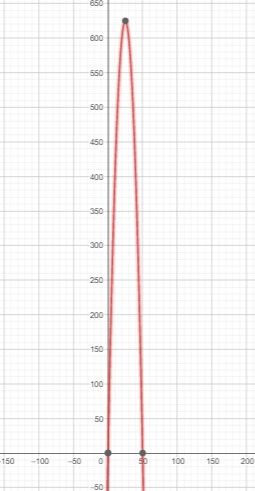
\includegraphics[width=5cm]{pics/1questao.jpeg} 
\caption{Gráfico da Função Área}
\end{figure}



















\newpage
\section{Questão:}
Suponha que a diminuição na pressão sanguínea de uma pessoa dependa
de determinada droga que ela deverá tomar. Assim, se x mg da droga forem
tomados , a queda da pressão será uma função de x. Seja $f(x)$ essa função e
$f(x) = \frac{1}{2}x^{2}(k - x)$ onde $x$ está em [0, k] , k constante. Calcule o valor de x que causa o maior decréscimo da pressão.

\begin{flalign*}
& f(x) = \frac{1}{2}x^{2}(k - x) & \\
& x \in [0, k] & 
\end{flalign*}

\subsection{Derivada da função}

\subsubsection{Derivada do produto com constante}
\begin{flalign*}
& f(x) = \frac{1}{2}x^{2}(k - x) & \\
& f(x) = \frac{1}{2}(kx^2 - x^3) & \\
& \frac{d f(x)}{d x} = \left(\frac{1}{2}(kx^2 - x^3)\right)' & \\
& \frac{d f(x)}{d x} = \frac{1}{2} \cdot (kx^2 - x^3)' & \\
\end{flalign*}

\subsubsection{Derivada da diferença}
\begin{flalign*}
& \frac{d f(x)}{d x} = \frac{1}{2} \cdot (kx^2 - x^3)' & \\
& \frac{d f(x)}{d x} = \frac{1}{2} \cdot ((kx^2)' - (x^3)') & \\
\end{flalign*}

\subsubsection{Derivada do expoente e da constante}
\begin{flalign*}
& \frac{d f(x)}{d x} = \frac{1}{2} \cdot ((kx^2)' - (x^3)') & \\
& \frac{d f(x)}{d x} = \frac{1}{2} \cdot (2kx - (x^3)') & \\
& \frac{d f(x)}{d x} = \frac{1}{2} \cdot (2kx - 3x^2) & \\
\end{flalign*}

\subsubsection{Derivada Final}
\begin{flalign*}
& \frac{d f(x)}{d x} = \frac{1}{2} \cdot (2kx - 3x^2) & \\
& \frac{d f(x)}{d x} = kx - \frac{3x^2}{2} & \\
\end{flalign*}

\subsection{Pontos Críticos}
Como queremos um ponto de máximo decréscimo de pressão iremos utilizar a análise  da derivada de f(x) para assim, por meio do coeficiente angular dado pela derivada, descobrirmos se naquele ponto existe um máximo ou não. Teremos alguns candidatos para serem a o x ponto de máximo decréscimo ( os números críticos ), neste caso como se trata de um intervalo fechado, os extremos são incluídos. \\ \\
Números críticos= $\{0, k\}$

\subsubsection{Achando quem zera}
Agora vamos descobrir quem zeraria esta derivada, significando que o coeficiente angular da reta tangente deste ponto seria 0, estando este paralelo ao eixo x e sendo então um máximo ou mínimo da imagem da função.

\begin{flalign*}
& \frac{d f(x)}{d x} = kx - \frac{3x^2}{2} & \\
& \frac{d f(x)}{d x} = 0 & \\
& \Rightarrow{kx - \frac{3x^2}{2} = 0} & \\
& \Rightarrow{kx = \frac{3x^2}{2} } & \\
& \Rightarrow{kx = \frac{3}{2} \cdot x^2 } & \\
& \Rightarrow{\frac{kx}{x^2} = \frac{3}{2}} & \\
& \Rightarrow{\frac{k}{x} = \frac{3}{2}} & \\
& \Rightarrow{k = \frac{3}{2} \cdot x} & \\
& \Rightarrow{x = \frac{2}{3} \cdot k} & \\
\end{flalign*}
Números críticos= $\{0, \frac{2k}{3} , k\}$


\subsubsection{Achando quem torna inexistente}
Podemos descobrir os pontos críticos quando nossa derivada é inexistente em determinada abscissa. Como esta derivada se trata de um polinônio simples, logo ela é definida para todos os pontos, então não haverão números críticos indicados por uma inexistência.

\subsubsection{Testando críticos}
Números críticos= $\{0, \frac{2k}{3} , k\}$
\begin{flalign*}
& f(x) = \frac{1}{2}x^{2}(k - x) & \\ \\
& f(0) = \frac{1}{2}0^{2}(k - 0) \Rightarrow{f(0) = 0 } & \\ \\
& f\left(\frac{2k}{3}\right) = \frac{1}{2} \cdot \left(\frac{2k}{3}\right)^{2} \cdot \left(k - \frac{2k}{3}\right)  \Rightarrow{f\left(\frac{2k}{3}\right) = \frac{1}{2} \cdot \frac{4k^2}{9} \cdot \frac{k}{3}} \Rightarrow{f\left(\frac{2k}{3}\right) = \frac{4k^3}{54}}  \text{ (Máximo)} & \\ \\
& f(k) = \frac{1}{2}k^{2}(k - k) \Rightarrow{f(k) = \frac{k^{2}}{2} \cdot 0 } \Rightarrow{f(k) = 0}  & \\
\end{flalign*}

\subsection{Conclusão}
Sendo assim o valor de x para que cause o maior decréscimo de pressão será $\frac{2k}{x}$ mg.
































\newpage
\section{Questão:}
Analise a função $f(x) = \frac{1}{4}x^4 - 2x^3 + 3x^2 + 2$, destacando os
pontos críticos ; \\
os intervalos onde f cresce e onde f decresce ; \\
intervalos onde a concavidade é positiva e intervalos onde essa concavidade é
negativa; \\ 
pontos de inflexão e assíntotas verticais e horizontais se
essas existirem.

\begin{flalign*}
& f(x) = \frac{1}{4}x^4 - 2x^3 + 3x^2 + 2 & \\
\end{flalign*}


\subsection{Análise da derivada - Pontos Críticos}

Como queremos um ponto crítico iremos utilizar a análise  da derivada de f(x) para assim, por meio do coeficiente angular dado pela derivada, descobrirmos se naquele ponto existe um ponto crítico ou não.

\subsection{Derivada de primeira ordem}
\begin{flalign*}
& \frac{d f(x)}{d x} = \left(\frac{1}{4}x^4 - 2x^3 + 3x^2 + 2\right)' & \\
\end{flalign*}

\subsubsection{Derivada da soma}
\begin{flalign*}
& \frac{d f(x)}{d x} = \left(\frac{1}{4}x^4\right)' - (2x^3)' + (3x^2)' + (2)' & \\
\end{flalign*}

\subsubsection{Derivada da constante}
\begin{flalign*}
& \frac{d f(x)}{d x} = \left(\frac{1}{4}x^4\right)' - (2x^3)' + (3x^2)' + 0 & \\ \\
& \frac{d f(x)}{d x} = \left(\frac{1}{4}x^4\right)' - (2x^3)' + (3x^2)' & \\
\end{flalign*}

\subsubsection{Derivada do produto com constante}
\begin{flalign*}
& \frac{d f(x)}{d x} = \frac{1}{4} \cdot (x^4)' - 2 \cdot (x^3)' + 3 \cdot (x^2)' & \\
\end{flalign*}

\subsubsection{Derivada do expoente}
\begin{flalign*}
& \frac{d f(x)}{d x} = \frac{1}{4} \cdot (4x^3) - 2 \cdot (3x^2) + 3 \cdot (2x) & \\ \\
& \frac{d f(x)}{d x} = x^3- 6x^2 + 6x & \\ 
\end{flalign*}

\subsection{Números críticos}
\subsubsection{Achando quem zera}
Agora vamos descobrir quem zeraria esta derivada, significando que o coeficiente angular da reta tangente deste ponto seria 0, estando este paralelo ao eixo x e sendo então um máximo ou mínimo da imagem da função.
\begin{flalign*}
& \frac{d f(x)}{d x} = x^3- 6x^2 + 6x & \\ 
& \Rightarrow{\frac{d f(x)}{d x} = 0}  & \\
& \Rightarrow{x^3- 6x^2 + 6x = 0}  & \\ 
& \Rightarrow{(x) \cdot (x^2 - 6x + 6)= 0}  & \\ 
\end{flalign*}
Isto implica que qualquer um dos lados do produto pode ser zerado
\begin{flalign*}
&
\begin{cases} 
&  \Rightarrow{x = 0} & \\
& \text{ Ou }& \\
&  \Rightarrow{x^2 - 6x + 6 = 0 } &
\end{cases} &
\end{flalign*}
\\
Achando raízes de x para que o segundo membro do produto seja zerado.
\begin{flalign*}
& \highlight{x=\frac{-b\pm\sqrt{\Delta}}{2a}} & \\
& \highlight{\Delta = b^2-4ac} & \\
& x^2 - 6x + 6 = 0 & \\ 
& \Delta = 36-4 \cdot 1 \cdot 6 & \\ 
& \Delta = 12 & \\ 
& x=\frac{6\pm\sqrt{12}}{2} & \\
& x=3\pm\sqrt{3} & \\
\end{flalign*}
\\
Números críticos atualizados = $\{0, 3-\sqrt{3}, 3+\sqrt{3}\}$

\subsubsection{Achando quem torna inexistente}
Podemos descobrir os pontos críticos quando nossa derivada é inexistente em determinada abscissa. Como esta derivada se trata de um polinônio simples, logo ela é definida para todos os pontos, então não haverão números críticos indicados por uma inexistência.

\subsubsection{Testando críticos - Teste da derivada de primeiro grau}
Números críticos = $\{0, 3-\sqrt{3}, 3+\sqrt{3}\}$
\begin{flalign*}
& f(x) = \frac{1}{4}x^4 - 2x^3 + 3x^2 + 2 & \\ \\
& f(0) = \frac{1}{4}\cdot0^4 - 2\cdot0^3 + 3\cdot0^2 + 2 = 2 & \\
& f(3-\sqrt{3}) \displaystyle \cong f(1,268) = \frac{1}{4}(1,268)^4 - 2(1,268)^3 + 3(1,268)^2 + 2 \displaystyle \cong 3.39  \text{ (Máximo) } & \\
& f(3+\sqrt{3}) \displaystyle \cong f(4,732) = \frac{1}{4}(4,732)^4 - 2(4,732)^3 + 3(4,732)^2 + 2 \displaystyle \cong -17.39 \text{ (Mínimo) }& \\
\end{flalign*}

\subsubsection{Pontos Críticos}
Com isto é possível concluir que os pontos críticos da função são:
\begin{flalign*}
& P(3-\sqrt{3}, 3.39)  \text{ (Máximo) } & \\
& P(3+\sqrt{3}, -17.39) \text{ (Mínimo) }& \\
\end{flalign*}


\subsection{Análise da derivada de segunda ordem - Pontos de Inflexão}
Com a derivada de primeira ordem nos tornamos capazes de descobrir o coeficiente angular da reta que tangencia f(x) no ponto de abscissa x, f'(x)=0 nos indica que ali é um ponto crítico da função. Se a segunda derivada for positiva em x, ou seja, f''(x) $ > $ 0, então x é ponto de mínimo. Se a segunda derivada for negativa em x, ou seja, f''(x) $ < $ 0, então x é ponto de máximo. \\
Além de nos indicar se é máximo ou mínimo, a derivada de segunda ordem quando for igual a zero indica um ponto de inflexão, onde a concavidade da parábola muda de sinal.


\subsection{Derivada de segunda ordem}
\begin{flalign*}
& f(x) = \frac{1}{4}x^4 - 2x^3 + 3x^2 + 2 & \\
& \frac{d f(x)}{d x} = x^3- 6x^2 + 6x & \\ 
& \frac{d^2 f(x)}{d x^2} = (x^3- 6x^2 + 6x)' & \\ 
\end{flalign*}

\subsubsection{Derivada da soma e diferença}
\begin{flalign*}
& \frac{d^2 f(x)}{d x^2} = (x^3)'- (6x^2)' + (6x)' & \\ 
\end{flalign*}

\subsubsection{Derivada do expoente e da constante}
\begin{flalign*}
& \frac{d^2 f(x)}{d x^2} = 3x^2- 12x + 6 & \\ 
\end{flalign*}

\subsection{Encontrando pontos de inflexão}
Onde a derivada de segunda ordem se torna zero.
\begin{flalign*}
& \frac{d^2 f(x)}{d x^2} = 0 & \\
& \Rightarrow{3x^2- 12x + 6 = 0} & \\
\end{flalign*}
\\
Achando raízes da equação de segundo grau
\begin{flalign*}
& \highlight{x=\frac{-b\pm\sqrt{\Delta}}{2a}} & \\
& \highlight{\Delta = b^2-4ac} & \\
& 3x^2- 12x + 6 = 0 & \\ 
& \Delta = 144 -4 \cdot 3 \cdot 6 & \\ 
& \Delta = 72 & \\ 
& x=\frac{12\pm\sqrt{72}}{6} & \\
& x=2\pm\sqrt{2} & \\
\end{flalign*}

\subsubsection{Pontos de Inflexão}
\begin{flalign*}
& f(2 + \sqrt{2}) \displaystyle \cong f(3,414) = \frac{1}{4}(3,414)^4 - 2(3,414)^3 + 3(3,414)^2 + 2 \displaystyle \cong -8.65 & \\ \\
& f(2 - \sqrt{2}) \displaystyle \cong f(0,585) = \frac{1}{4}(0,585)^4 - 2(0,585)^3 + 3(0,585)^2 + 2 \displaystyle \cong 2.65 & \\ \\
& P_{Inflexão 1}(2 + \sqrt{2}, -8.65) & \\
& P_{Inflexão 2}(2 - \sqrt{2}, 2.65) & \\
\end{flalign*}



\subsection{Análise - Crescimento, decrescimento e concavidade da parábola}
Analisando o sinal da derivada de primeira e de segunda ordem conseguimos visualizar como a imagem da função se desenvolve. 
\\ 
A derivada de primeira ordem nos indica o coeficiente angular, quando este é positivo indica que a função está crescendo, e quando é negativa indica que está decrescendo.
\\
A derivada de segunda ordem nos indica o sinal da concavidade da parábola no ponto.
\begin{figure}[h]
\centering
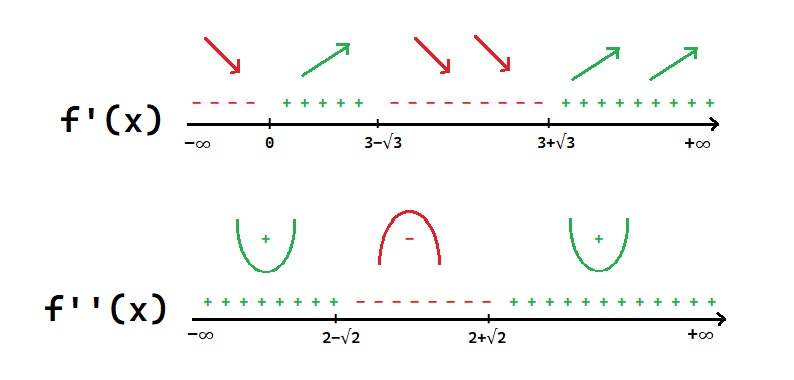
\includegraphics[width=10cm]{pics/analise.jpg} 
\caption{Análise da Função}
\label{figura:analise}
\end{figure}


\begin{figure}[h]
\centering
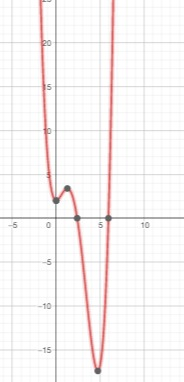
\includegraphics[width=5cm]{pics/3questao.jpeg} 
\caption{Gráfico de f(x)}
\end{figure}

\subsection{Análise de assíntotas}

\subsubsection{Assíntota horizontal}
A assíntota horizontal é encontrada quando tendemos o x ao infinito e descobrimos que o limite se torna uma constante.
\begin{flalign*}
& \highlight{lim_{x \to \pm \infty} f(x) = c} & \\
& lim_{x \to \pm \infty} f(x) = \frac{1}{4}x^4 - 2x^3 + 3x^2 + 2  & \\
\end{flalign*}
Utilizando da propriedade dos limites polinomiais quando a variável tende ao infinito onde apenas o monômio de maior expoente permanece.
\begin{flalign*}
& lim_{x \to \pm \infty} f(x) = \frac{1}{4}x^4  & \\
& lim_{x \to \pm \infty} f(x) = \pm \infty  & \\
\end{flalign*}
Quando x tende ao infinito, o limite de f(x) tende há um comportamente e não a uma constante, portanto f(x) não possui assíntota horizontal.

\subsubsection{Assíntota vertical}
A assíntonta vertical é encontrada quando em determinado x a função tender ao infinito.
\begin{flalign*}
& \highlight{lim_{x \to x_0} f(x_0) = \frac{k}{0} = \pm \infty} & \\
& \highlight{k \in \mathbb{R} \And k \neq 0} & \\
\end{flalign*}
Como nossa função f(x) se trata de um polinômio, logo ela é contínua e definida em todos os seus pontos, não possuindo assíntota vertical.



\end{document}